\documentclass[12pt]{article}

% Solution to underfull hbox warning
% Found at: https://tex.stackexchange.com/questions/10924/underfull-hbox-in-bibliography
\usepackage{etoolbox}
% Variant A
\apptocmd{\sloppy}{\hbadness 10000\relax}{}{}
% Variant B
% \apptocmd{\thebibliography}{\raggedright}{}{}

\usepackage{geometry}
\geometry{margin=1in}

\usepackage{graphicx}
\graphicspath{ {./images/} }

\usepackage{float}

\usepackage{helvet}
\renewcommand{\familydefault}{\sfdefault}

\usepackage{indentfirst}

\usepackage[labelfont=bf]{caption}

\usepackage{tocloft}
\renewcommand{\cftsecleader}{\cftdotfill{\cftdotsep}}

\usepackage{hyperref}
\hypersetup{
    colorlinks,
    citecolor=black,
    filecolor=black,
    linkcolor=black,
    urlcolor=black
}

\begin{document}

    \pagenumbering{gobble}

\noindent
Reza Rizvi

\noindent
Assistant Professor

\noindent
Department of Mechanical Engineering

\noindent
York University

\noindent
\\Dear Professor Rizvi,

\noindent
\\I have prepared the following report ``Machine Learning for Cybersecurity'' detailing a possible solution for the Engineering Grand Challenge of Securing Cyberspace.
This report will be ready for publishing by March 22, 2022.

\noindent
\\In this report I discuss the Engineering Grand Challenge of Securing Cyberspace and its associated problems.
I then offer as a solution the development of machine learning for cybersecurity, detailing its capabilities, strengths, weaknesses, and effectiveness in making progress for the grand challenge.
I intend for this report to educate and inform you of the importance of these issues and the suitability of the new technology.

\noindent
\\I encourage you to contact me if you have questions, concerns, or any feedback.
Thank you for your time.

\noindent
\\Sincerely,

\noindent
\\FirstName LastName
\\email@yorku.ca
\\(012) 345-6789


    \pagebreak

    \begin{titlepage}
    \begin{center}
        \vspace*{1cm}

        \Huge\textbf{Machine Learning for CyberSecurity}

        \vspace*{0.5cm}

        \LARGE A Solution to the Engineering grand Challenge of Securing Cyberspace

        \vspace*{1.5cm}

        \Large March 8, 2022

        \vfill

        
\includegraphics[width=0.7\textwidth]{YorkU_Logo.png}

        \vspace*{1cm}

        \large I attest that that this is my original work.
    \end{center}
\end{titlepage}

    \pagenumbering{roman}

\section*{Executive Summary}
\addcontentsline{toc}{section}{Executive Summary}
\setcounter{page}{2}
The internet is one of the most complex systems ever engineered.
Utilizing this complexity, cybercriminals have an abundance of opportunities to wreak havoc through the internet.
The options for attacks range from sending fake emails in an attempt to steal someone's password, to shutting down entire power grids.
As industries become more dependent on technology and the internet, the latter case is more feasible for cybercriminals.

The engineering grand challenge of securing cyberspace addresses this problem.
The challenge acknowledges that the massive scope of this problem, and that it will only get worse as technology dependence increases.
This challenge falls into the cross-cutting theme of security, which needs to be prioritized for these reasons.
Creating a secure cyberspace is necessary for the proper functioning of industry and prevention of costly damages.

An emerging technology that addresses this grand challenge is machine learning.
Machine learning models can be trained using training data to detect patterns in new data.
This is especially useful for this challenge, as current pattern recognition software for cybersecurity is programmed manually and is unable to keep up with constantly changing cyberattacks.
Machine learning has an opportunity here to provide automatic detection of malicious activity that can evolve along with the evolving threats.

Initial tests and implementations of this technology are promising.
MalDozer, a machine learning malware detection system for the Android operating system, has shown in experiments to be about 96\% accurate with a false positive rate of about 2\%.
Outside of experiments, the Windows Defender Antivirus, an antivirus software developed by Microsoft, has already implemented machine learning in its production software.
It has faced a cyberattack targeting over one thousand Windows users, to which it correctly identified malicious activity and blocked the attack.

Although promising, the machine learning's use for cybersecurity currently has some drawbacks.
One drawback is that there is not enough datasets to train the machine learning models with.
If not properly trained, the models will not be effective in detecting malicious activity.
Also, while machine learning receives much research, most of it is not directed to cybersecurity.
As a result, the technology still needs to be researched before it can be widely adopted.

Despite these drawbacks, machine learning is a promising solution for the grand challenge.
With more research and resources, this technology will be capable of solving much of the challenge and secure a large part of cyberspace.


    \pagebreak

    \tableofcontents

    \pagebreak

    \addcontentsline{toc}{section}{List of Figures}
\listoffigures


    \pagebreak

    \pagenumbering{arabic}

    \section{Introduction and Background}
Technology and the internet have been growing more and more pervasive over the last few decades, and this shows no sign of stopping.
This comes with many benefits, like an abundance of readily available information, almost instantaneous communication, and the entire industry of online markets.
However, this also comes with consequences.
Perhaps one of the most pressing issues with the growth of technology is the introduction of a new type of malicious activity---cybercrime.

Cybercrime is the use of the Internet for illegal purposes.
This includes crimes targeting individuals, such as malware, ransomware, phishing, and identity theft.
But with the increasing dependance of industry on the internet, this cybercrime includes crimes that target populations and large systems.
For example, cyberattacks can target entire organizations, power grids, military systems.

The engineering grand challenge of securing cyberspace seeks to address this problem.
The internet is one of the most complex systems ever engineered, and the complexity of the internet leads to complexity in the cyberattacks that threaten it.
Falling under the cross-cutting theme of security, this grand challenge acknowledges the massive scope of this problem.
It acknowledges the possibly devastating effects of cyberattacks and costly consequences.

Such cyberattacks have happened.
On June 1, 2020, the University of California, San Francisco, was hacked by a ransomware campaign that threatened to release confidential information, to which the university paid approximately \$1.14 million to the group \cite{winder2020}.
In fact, in 2015, cybercrime was estimated to have had a global cost of \$3 trillion \cite{microsoft2016}, and is predicted to reach \$10.5 trillion by 2025 \cite{morgan2020}.

As is evident by successful cyberattacks of reputable organizations, current methods of dealing with these attacks are insufficient.
The main method of developing cybersecurity systems is quickly finding fixes when a successful cyberattack occurs.
Clearly, a much more proactive and complex cybersecurity system is needed to deal with this.


    \section{Machine Learning's Use in Cybersecurity}
% Cybersecurity systems include many different systems, like firewalls and antivirus software.
% Once such type is called an intrusion detection system (IDS).
% IDSs help to differentiate between authorized and unauthorized uses of a provided service \cite{xin2018}.
% This is a technology that machine learning has the most potential to impact.

Traditionally, cybersecurity algorithms were written manually from heuristics \cite{sarker_kayes_badsha_2020}.
But the rapid growth of the internet and technology in general has led to constantly changing cybersecurity threats.
As a result, these manually written heuristic algorithms are insufficient --- they cannot keep up with the evolving threats \cite{sarker_kayes_badsha_2020}.
Machine learning offers a solution to this problem.

Machine learning models are able to ``learn'' certain data patterns to predict behavior \cite{sarker_kayes_badsha_2020}.
In this case, their goal is to predict whether some online activity is malicious or legitimate.
To accomplish this, the model must be trained with training data and tested to ensure it is effective.
This first involves data-driven tasks, like gathering and cleaning data \cite{sarker_kayes_badsha_2020}.
This data can then be used to train the model, which may take seconds to days, depending on the algorithm chosen \cite{xin2018}.
Once the model is trained, it must be tested to ensure it is accurately detecting malicious activity, which also takes a variable amount of time depending on the machine learning algorithm chosen \cite{xin2018}.
Figure 1 shows a diagram of this process.

\begin{figure}[H]
    \centering
    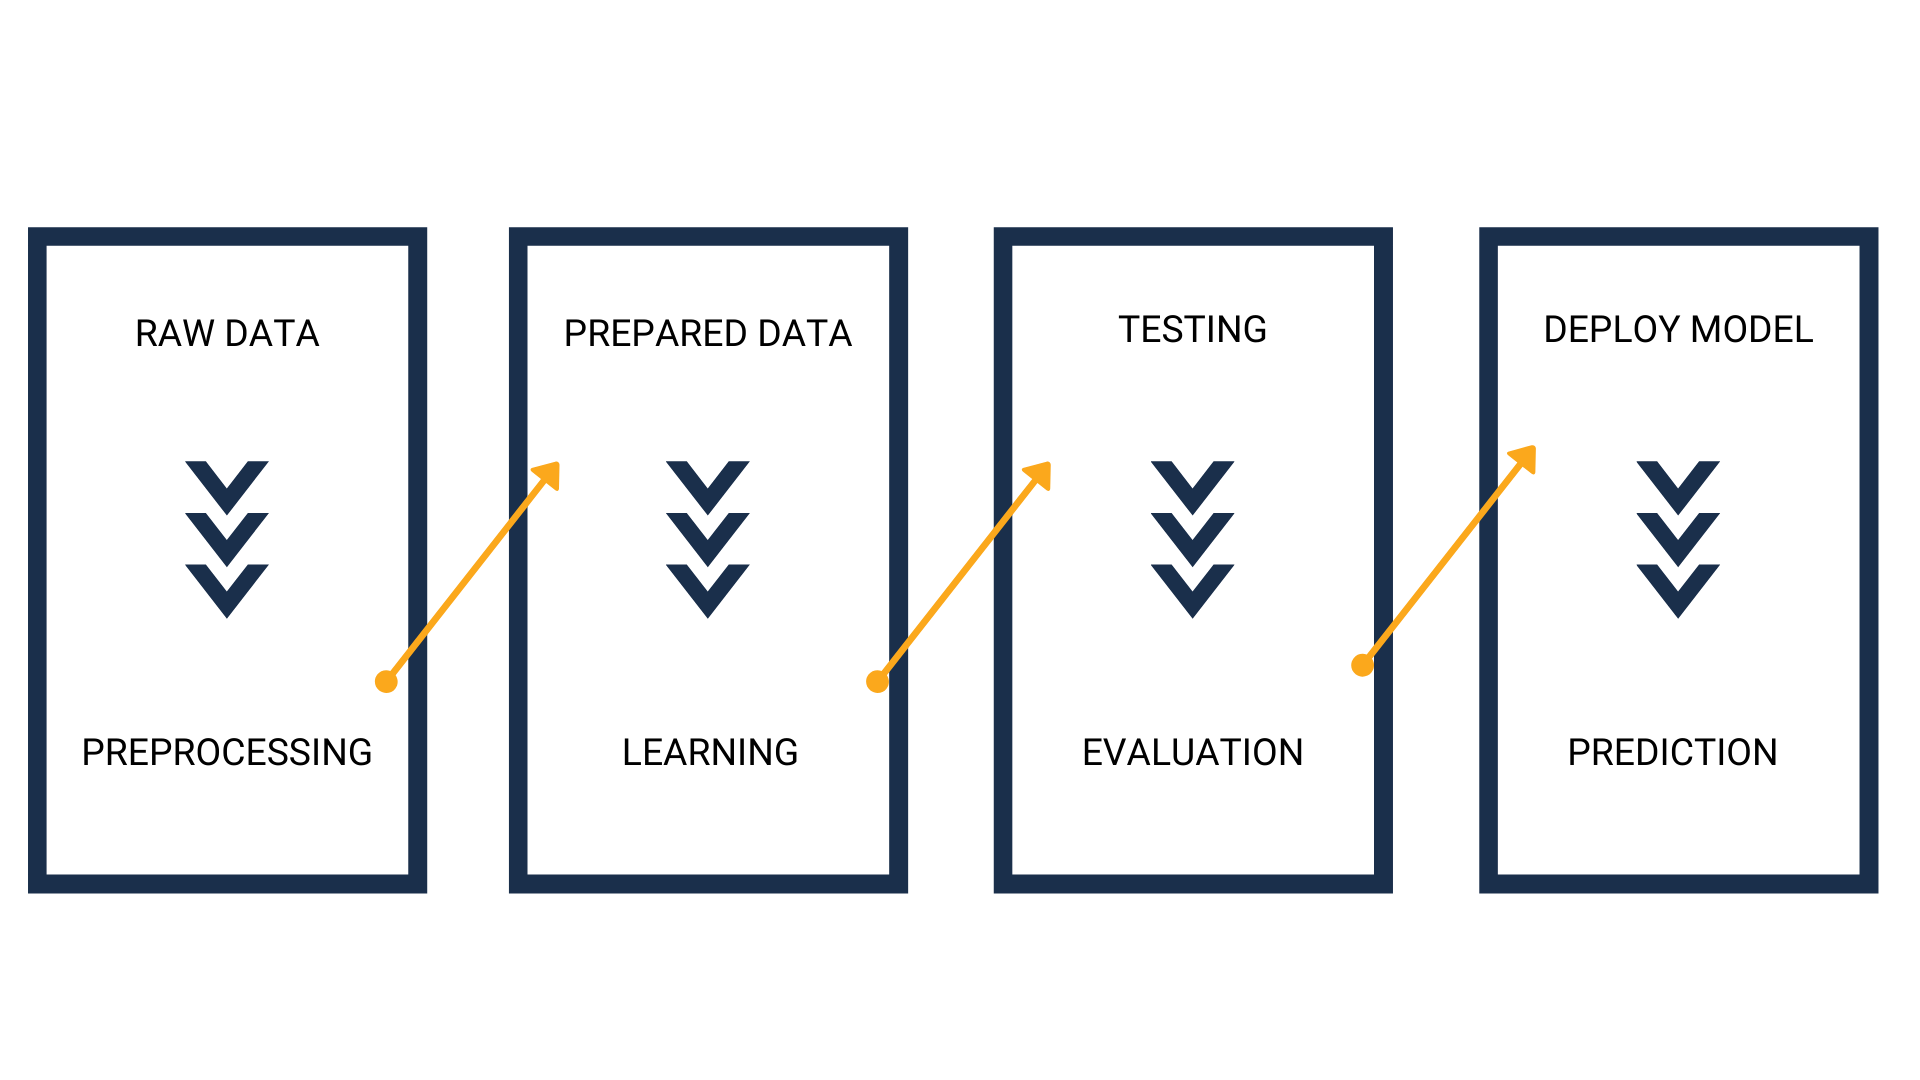
\includegraphics[width=0.7\textwidth]{echosec_machine_learning_diagram.png}
    \caption{A Diagram of a Typical Machine Learning Process. \cite{echosec}}
\end{figure}

\section{Evidence of Machine Learning's Effectiveness}
Machine learning algorithms are already being employed to detect cyberattacks.
The following are a few case studies of machine learning being successfully implemented.

\subsection{Windows Defender Antivirus}
In 2018, a new malware attack campaign was launched against over a thousand users of Windows 7 Pro \cite{microsoft2018}.
The Windows Defender Antivirus features lightweight machine learning models built into the client, which responded immediately to the attack \cite{microsoft2018}.
These models detected a high probability of maliciousness, so they sent data to the Windows Defender Antivirus cloud protection service, which runs more complex machine learning models \cite{microsoft2018}.
Through this, the cloud protection service correctly identified the requests as a cyberattack and responded back to the clients, instructing them to block the attack \cite{microsoft2018}.
The use of machine learning algorithms were able to protect thousands of users from a cyberattack with no human intervention.

\section{Drawbacks of Machine Learning for Cybersecurity}
In its current state, machine learning has many drawbacks for use in cybersecurity, some of which make it infeasible for organizations to use.

\subsection{Availability of Datasets}
Since cyberattacks can be complex and varied, large datasets are needed to train the machine learning models to ensure they can protect against all attacks.
This is not the case with the existing datasets available.
Current datasets contain lots of old data and redundant information \cite{xin2018}.
This can be somewhat improved after cleaning the data, but even then there is the issue of volume --- there is not enough data to properly train the models \cite{xin2018}.
As a result, the machine learning models are not totally equipped for identifying new cyberattacks.
This also introduces a barrier of entry, as larger organizations may be able to work around these issues, but smaller organizations do not have the resources to do so.

\subsection{Lack of Research and Adoption}
While the field of machine learning receives lots of research, this research is mainly focused on deep-learning algorithms for applications like self-driving cars \cite{grandchallenge2019}.
Machine learning for cybersecurity purposes has yet to receive this same amount of attention.
Due to this lack of research, widely adopted machine learning models for cybersecurity are limited, using mostly rule-based techniques \cite{grandchallenge2019}.
Furthermore, this lack of research introduces inconsistency across organizations \cite{grandchallenge2019}.
To be most effective, cybersecurity models need to have consistent behavior for any attack that may occur.
This requires cooperation and research to keep all parts of the internet secure.

\section{Discussion}


    \pagebreak

    \section{Conclusion}
The engineering grand challenge of securing cyberspace has a level of complexity and difficulty that is daunting.
However, this complexity and difficulty can be matched with machine learning.

With the ability to find patterns in data, machine learning shows potential as a detection system for malicious activity.
Even though the cyberthreats it must respond to are constantly evolving, machine learning models will remain effective because they can evolve with the threats.
This has been shown both in experimental settings and in real cyberattacks.

In its early stages, this technology is proving to be accurate and effective, and this will only improve with research.
As barriers to entry fade and more research and datasets are compiled, machine learning will be imperative for securing cyberspace.


    \pagebreak

    \begin{thebibliography}{99}
    \bibitem{winder2020}
    D. Winder, ``The University Of California Pays \$1 Million Ransom Following Cyber Attack,''
    \textit{forbes.com}, Jun. 29, 2020. [Online].
    Available: \href{https://www.forbes.com/sites/daveywinder/2020/06/29/the-university-of-california-pays-1-million-ransom-following-cyber-attack/?sh=5628ae8618a8}{https://www.forbes.com/sites/daveywinder/2020/06/29/the-university-of-california-pays-1-million-ransom-following-cyber-attack/?sh=5628ae8618a8}
    [Accessed March 6, 2022].

    \bibitem{microsoft2016}
    Microsoft Secure Blog Staff, ``The Emerging Era of Cyber Defense and Cybercrime,''
    \textit{Microsoft}, Jan. 27, 2016. [Online].
    Available: \href{https://www.microsoft.com/security/blog/2016/01/27/the-emerging-era-of-cyber-defense-and-cybercrime/}{https://www.microsoft.com/security/blog/2016/01/27/the-emerging-era-of-cyber-defense-and-cybercrime/}
    [Accessed March 7, 2022].

    \bibitem{morgan2020}
    S. Morgan, ``Cybercrime To Cost The World \$10.5 Trillion Annually By 2025,''
    \textit{cybersecurityventures.com}, Nov. 13, 2020. [Online].
    Available: \href{https://cybersecurityventures.com/cybercrime-damages-6-trillion-by-2021/}{https://cybersecurityventures.com/cybercrime-damages-6-trillion-by-2021/}
    [Accessed March 7, 2022].

    \bibitem{sarker_kayes_badsha_2020}
    I.H. Sarker, A.S.M. Kayes, S. Badsha, ``Cybersecurity data science: an overview from machine learning perspective,''
    J Big Data, Jul. 1, 2020. [Online].
    Available: \href{https://doi.org/10.1186/s40537-020-00318-5}{https://doi.org/10.1186/s40537-020-00318-5}
    [Accessed February 28, 2022].

    \bibitem{xin2018}
    Y. Xin et al., ``Machine Learning and Deep Learning Methods for Cybersecurity,''
    \textit{IEEE Access}, vol. 6, pp.3 5365-35381, 2018. [Online].
    Available: \href{https://ieeexplore.ieee.org/abstract/document/8359287/citations?tabFilter=papers}{https://ieeexplore.ieee.org/abstract/document/8359287/citations?tabFilter=papers}
    [Accessed March 7, 2022].

    \bibitem{echosec}
    Echosec Systems, ``How Is Machine Learning Used in Cybersecurity?,''
    \textit{Echosec Systems}. [Online].
    Available: \href{https://www.echosec.net/blog/how-is-machine-learning-used-in-cybersecurity}{https://www.echosec.net/blog/how-is-machine-learning-used-in-cybersecurity}

    \bibitem{microsoft2018}
    Microsoft Defender Security Research Team, ``How artificial intelligence stopped an Emotet outbreak,''
    \textit{Microsoft}, Feb. 14, 2018. [Online].
    Available: \href{https://www.microsoft.com/security/blog/2018/02/14/how-artificial-intelligence-stopped-an-emotet-outbreak/}{https://www.microsoft.com/security/blog/2018/02/14/how-artificial-intelligence-stopped-an-emotet-outbreak/}
    [Accessed March 7, 2022].
\end{thebibliography}


    \pagebreak

    \section*{Appendix A: Feedback Summary}
\addcontentsline{toc}{section}{Appendix A: Feedback Summary}
The summary of the feedback from each of the three peers is summarized below, along with the actions I chose to take given the feedback.

\subsection*{Peer 1}
\addcontentsline{toc}{subsection}{Peer 1}
The feedback from the first peer mentioned some errors with grammar and sentence flow.
They annotated the report to point out these errors, most of which I agreed with and fixed.
One comment I did not agree with is that the reviewer mentioned not capitalizing the word Internet in the Introduction and Background section, where I write ``the Internet''.
I argue that this should be capitalized because I am referring to the Internet as a proper noun, not as an adjective.

The reviewer also noted that I did not include a List of Figures section, so I added that.


\end{document}
